% Copyright (C) 2001, International Business Machines
% Corporation, Ted Ralphs and others. All Rights Reserved.

\section{Directory Layout (location of the source files)}
\label{dev:source-files}

The easiest way to get oriented is to examine the organization of the
source files. Once you install the \BB\ distribution and enter the
\code{Bcp} directory, you will see several subdirectories, including
one called \code{Bcp-common/}. \code{Bcp-common/} contains the source
files for the internal framework. Users should not have to modify
these files, but should be familiar with their organization. The other
directories contain the source code for applications. There are two
samples available, a Max Cut solver (\code{MaxCut/}) and a solver for
the Multiple Knapsack Problem with Color Constraints (\code{Mkc/}).
First let's explore the Bcp-common directory.

Within \code{Bcp-common/}, there are directories associated with each
of the modules, a directory called \code{Member/} and a directory 
(\code{include/}) for the header files. The source files in \code{Member/}
contain the implementation of methods of classes that are used in
multiple modules (like cuts and variables), while the module
directories contain module specific class methods and module specific
functions.

The same directory hierarchy is used in the directories of the sample
applications and it is recommended that the user adheres to this
convention simply because the \code{Bcp/Makefile} automatically looks
for user source files in these directories. If the user places her
files in different directories then she must specify those directories
in \code{USER\_SRC\_PATH}.

\section{Overview of the Class Hierarchy}
\label{dev:overview-hierarchy}

We now briefly describe the class hierarchy from the user's point of view. Our
aim here is not to describe the full class structure, but just those parts
that the user needs to be familiar with in order to derive new user classes
and override the appropriate methods. As we discussed in Chapter
\ref{man-intro}, we have taken an object-oriented approach with the main
objects being the cuts and variables. As such, there are three main
``object'' classes from which the user may want to derive new
problem-specific descendents. These are:
\begin{itemize}
\item \code{BCP\_cut}: This class is used for describing cuts. There are three
  child classes derived from this one which implement the three
  different types of cuts---core, indexed, and algorithmic.
\item \code{BCP\_var}: This class is used for describing variables. Again,
  there 
  are three derived classes which implement the three different types
  of variables---core, indexed, and algorithmic.
\item \code{BCP\_solution}: This class is used for describing feasible
  solutions to the full problem. This description may be implemented
  simply as a list of the nonzero variables and their corresponding
  values or can be a user-defined representation of a more
  combinatorial nature. For instance, in the Traveling Salesman
  Problem, the user may wish to store feasible solutions directly as
  permutations of the nodes instead of just as a list of edge variable
  indices and values.
\end{itemize}
Ideally, these would be the only classes the user would need to worry
about. However, in order to modularize the code and support
parallelism, we have deviated from an idealized, object-oriented
design and defined some module-oriented ``interface'' classes as well.
These classes do not contain any data elements, but instead contain
methods which are unique to a particular module and cannot be
contained in one of our primary object classes. They also contain
methods which work on sets of objects---these cannot be implemented in
the standard, object-oriented fashion. As an example, all the
subroutines for communicating data between the modules. The interface
classes are:
\begin{itemize}
\item \code{BCP\_xx\_user}: Here, ``xx'' is the name of a particular module.
  The 
  user must derive a new class for each module in which she wants to
  override a default method. Note that although these base classes
  exist primarily as containers for module-specific methods, the user
  can also use his derived classes to store the problem data needed
  for performing the user-defined methods in that module.
  Alternatively, these data structures could be defined in a separate
  base class and then, using multiple inheritance, derived into a
  common child class.
\item \code{USER\_initialize}: This class contains subroutines for generating
  objects from the derived interface classes. This is also where the
  messaging environment and LP solver environment objects are created.
\end{itemize}
In addition to deriving from these classes as appropriate, the user must also
provide the definition of the function called \code{BCP\_user\_init()} which
returns an object of the 
class derived from \code{USER\_initialize}.

\section{The Flow of the Algorithm}

Keeping in mind this basic class structure, we now describe again, as
in Chapter \ref{man-intro}, the overall flow of the BCP algorithm, but
this time with more detail and an emphasis on how the interface
routines defined in the \code{BCP\_xx\_user} classes fit into this
flow. In some cases, it may be important to know the specific order in
which the interface routines are called since procedures performed in
one subroutine could depend on data generated in a previous
subroutine. This applies mainly to the LP module, which has the
largest number of associated interface routines.

%We will describe which methods the user can
%override in each module class and in which order those methods are invoked.
%This latter information is useful in case she wants to precompute something in
%one method and return results in another. For example, while testing
%feasibility she might find violated cuts she would want to report when cut
%generation is requested. Note that the user need not override all methods she
%can, indeed, for most problems she would want to override only a small
%fraction of the methods (see Table \ref{xxx}).

In Figures \ref{dev:initmodule} and \ref{dev:lploop}, 
the arrows between boxes indicate the flow
of the algorithm. Keep in mind that these charts merely give a
high-level description of the algorithm. Section
\ref{dev:user-derived} and the HTML documentation contain a full and
detailed description of the API. Figure \ref{dev:initmodule} indicates
how the solver is initialized and lists the interface routines used by
the tree manager, the cut generator, and the variable generator.
First, the solver environment is initialized (see Section
\ref{dev:USER_initialize}), then the module-specific user classes are
created. Afterwards, the user specifies the initial set of core and
extra variables and packs the problem data to be sent to the other
modules. Initialization of each of the slave processes begins with the
unpacking of these data at their destinations.

Once the solver is initialized, the TM module utilizes only three
interface methods. The first one initializes a new phase (see Section
\ref{two-phase}), the second receives a new feasible solution, while
the third compares two search tree nodes. This comparison function is
used to insert new candidate nodes into a priority queue. The top
element of the queue will be selected for processing when an LP
process becomes available. Similarly, the CG and VG modules also call
relatively few interface routines. Their only job is to wait for a
primal (dual) solution from which they try to generate violated valid
inequalities (improving columns). The generated objects are sent back
to the LP process.Figure (\ref{dev:lploop}) describes the flow of
the LP solver loop, from where the majority of the interface routines
are called. These routines will be described below.

\begin{figure}
\begin{center}
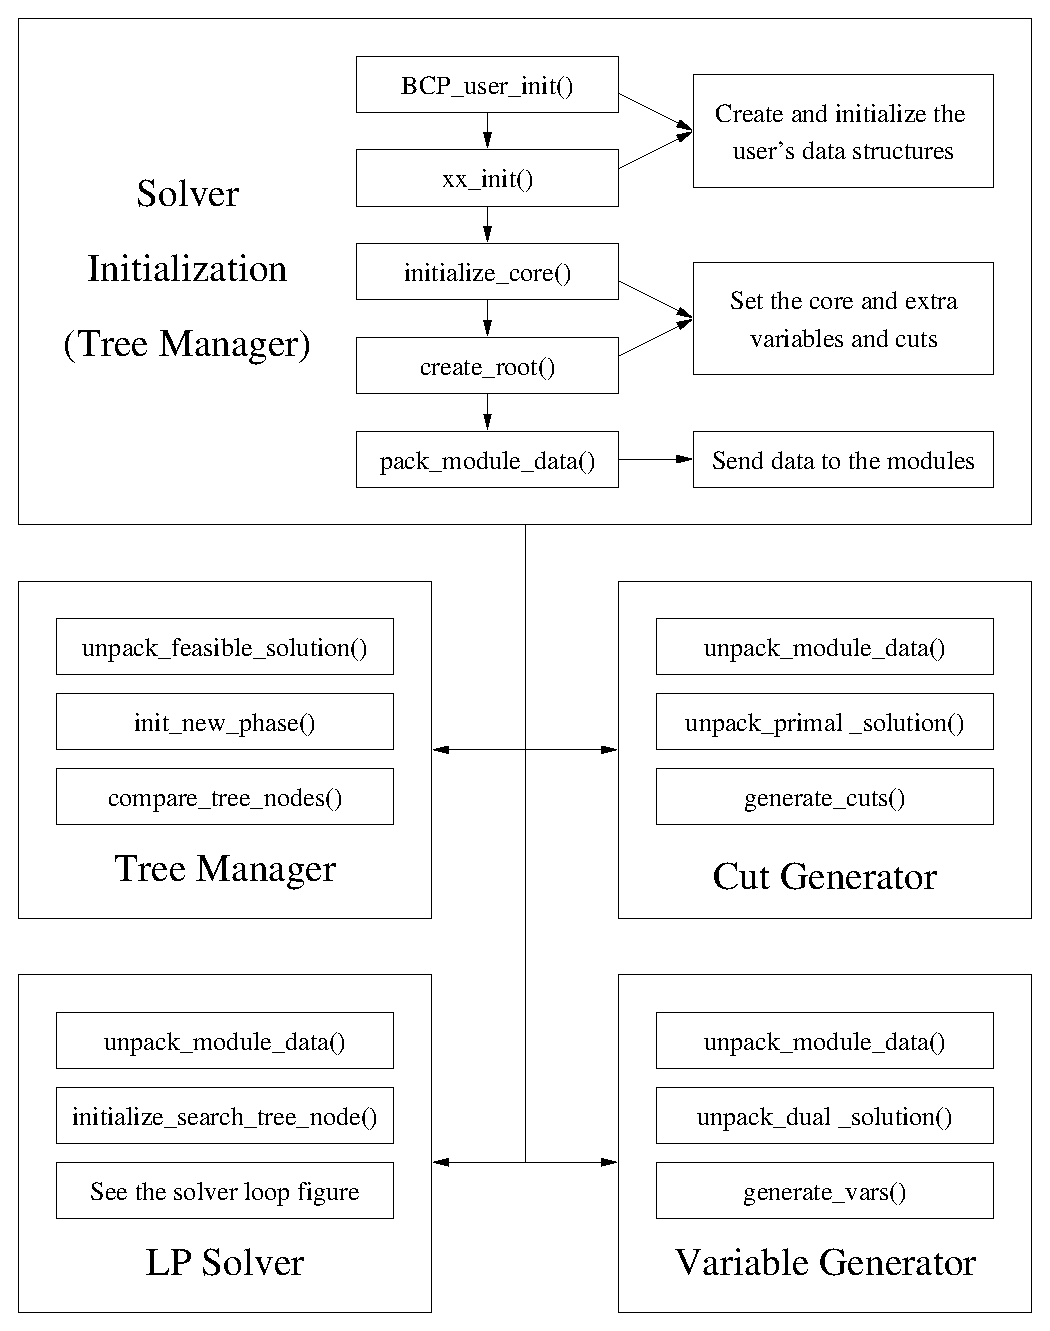
\includegraphics[scale=0.75]{flow-init.eps}
\end{center}
\caption{\label{dev:initmodule} Solver initialization and algorithm overview}
\end{figure}

\begin{figure}
\begin{center}
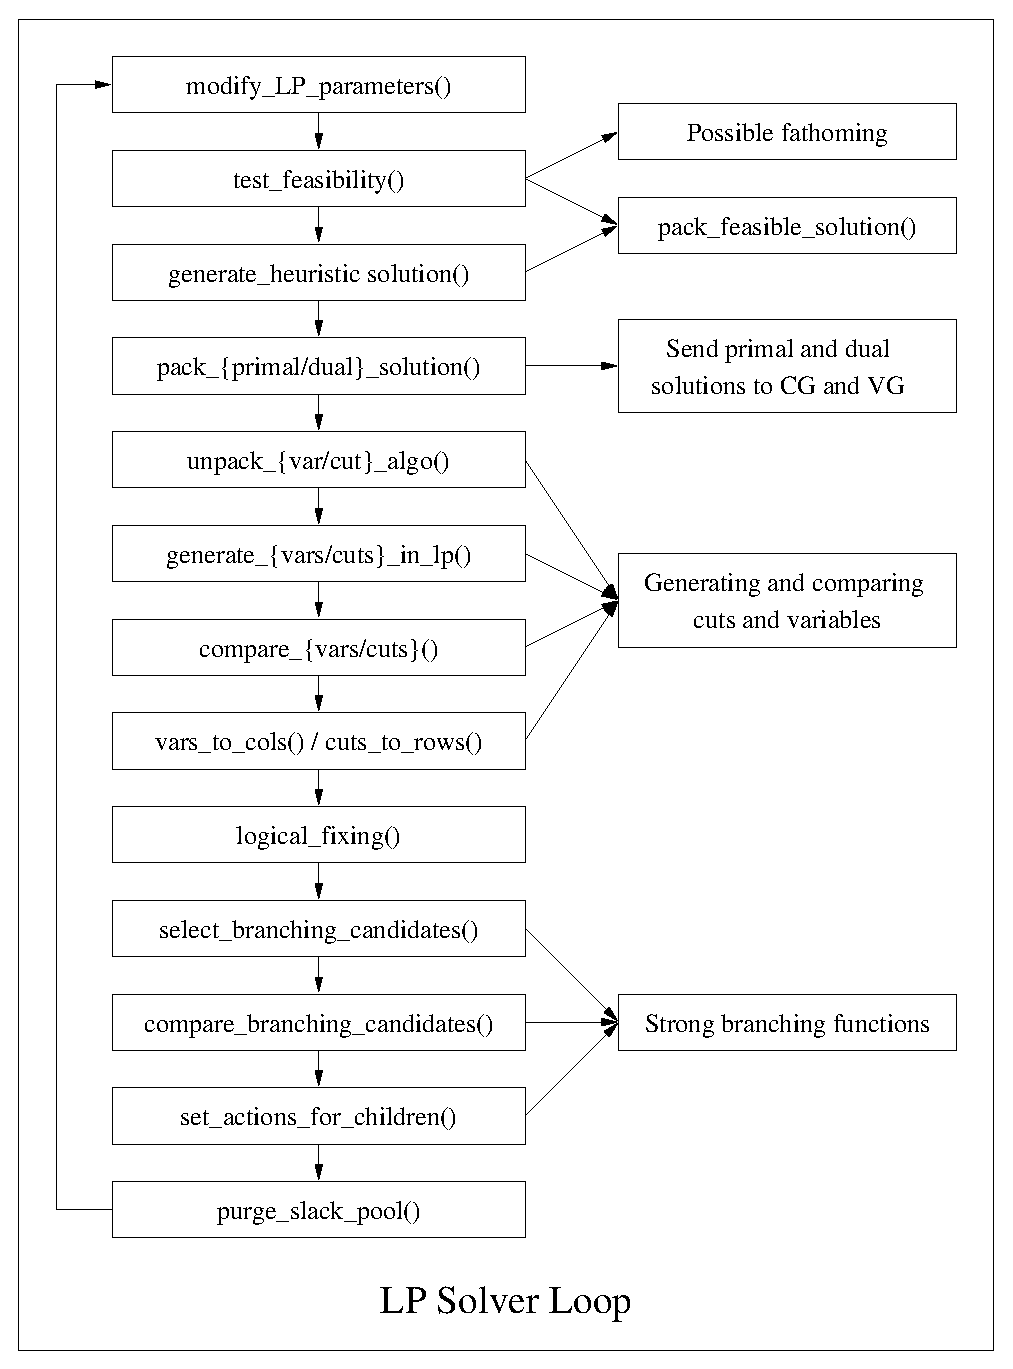
\includegraphics[scale=0.75]{flow-lploop.eps}
\end{center}
\caption{\label{dev:lploop}LP solver loop}
\end{figure}

\subsection{Fathoming procedure}

Fathoming, which is very simple
in a regular branch and cut algorithm is much more involved when
pricing is present. The reason is that introducing new columns can
push the lower bound below the global upper bound or can restore
feasibility if the LP relaxation was found infeasible. If a true
optimal solution is desired in a BCP algorithm, then a search tree
node can be fathomed if and only if there are no columns that can
restore feasibility and there is no column with negative reduced cost.
Of these two conditions the first one is the ``worse''. Almost always
there are variables that can be introduced to restore feasibility, but
usually that pushes the lower bound too high. However, we {\em must}
restore feasibility, because there can be columns with negative
reduced cost afterwards that could bring down the objective value. On
the other hand, when fathoming would happen because of too high lower
bound, all we got to look for are columns with negative reduced cost.
Frequently none are found (especially if the global upper bound is
really good) so the node can really be fathomed. For this reason it is
recommended that users wanting to generate variables on the fly set up
their model in a way that ensures primal feasibility at all times.
(Not to mention that then she doesn't have to override the feasibility
restoration methods.)

For each search tree node \BB\ maintains a state, that is, whether there are
indexed or algorithmic variables not in the formulation. Furthermore, for
indexed variables \BB\ can maintain a list about which ones have been
permanently priced out (excluded from any solution in the subtree). To utilize
this ability of \BB, only two very simple methods must be overridden:
\code{next\_indexed\_var()} and \code{create\_indexed\_var()}. The first
method is 
used to enumerate the indices of the indexed variables one by one, the second
method is used to actually create the indexed variables.

Now if fathoming would happen because the lower bound exceeds the upper bound
then, if \BB\ is instructed to maintain the above mentioned list, first the
not-yet-priced-out indexed variables are tested then the 
\code{generate\_vars\_in\_lp()} method is invoked for finding algorithmic
variables with negative reduced cost. 

If fathoming would happen because of infeasibility then again first the
indexed variables tested whether any of them destroys the proof of
infeasibility (i.e., whether it has a negative inner product with the
specified dual ray) then the \code{restore\_feasibility()} method is invoked so
that the user can test the algorithmic variables.

\section{Details of the Interface}
\label{dev:user-derived}

As mentioned earlier in our overview of the class hierarchy (Section
\ref{dev:overview-hierarchy}), the user can modify the behavior of the
framework by overriding the default methods. To override the methods
in a particular module, she simply derives a new child class from the
corresponding \code{BCP\_xx\_user} base class and overrides the
appropriate methods. If not overridden, the default method will be
invoked by the framework. Whenever possible, methods have default
which will work for the most common problem settings. In some cases,
there are several default implementations from which the user can
choose by setting a parameter. Alternatively, these methods can
be invoked directly by the user as desired, allowing for the use of
different methods in different situations. In the remainder of this
section, we describe in more detail the virtual methods of the
interface classes. These descriptions are at a high level---for the
exact specification, see the HTML manual pages included with the
distribution \cite{HTML-manual}.

\subsection{The \code{USER\_initialize} class}
\label{dev:USER_initialize}

The user must communicate the existence of the objects she designed to
\BB. For example, for all processes she intends to use she must have
derived something from the \code{BCP\_xx\_user} classes. Since \BB\
contains the \code{main()} function there are two ways to achieve this.
The ``C'' style solution is to have a functions declared in \BB\ but
not defined. These functions must be defined by the user and return
pointers to objects defined by her. The disadvantage of this solution
is that the user has to define all of these functions, even if she
doesn't intend to create some type of objects. Furthermore, if there
are possible defaults she must indicate somehow to the calling
function that a default should be executed.

\BB\ employs a C++ style coding here. Only one function is declared that the
user must define, \code{BCP\_user\_init()}. This function must
return an object of a type she derived from \code{USER\_initialize} and
in which she overrode some methods. This way the user is forced to
define only one function, and she can choose the default behavior
(like initializing the LP engine class) by simply not overriding a
method.

When \BB\ will be converted into a library there will be no need for this
class. 

\begin{itemize}
\item \code{msgenv\_init()}: return the message passing environment to be used.
  The user probably doesn't want to override this method, as the default 
  \BB\ uses will be determined by the value of \code{COMM\_PROTOCOL} in the
  application Makefile.
\item \code{tm\_init()}: return the object the user has derived from 
  \code{BCP\_tm\_user}. Note that this method should also take care of reading
  the parameter file and the problem data and whatever initialization the user
  wants to do. The user {\em must} override this method, there {\em must} be a
  user derived tree manager class.
\item \code{lp\_init()}: return the object the user has derived from 
  \code{BCP\_lp\_user}. The user {\em must} override this method, there 
  {\em must} be a user derived LP class.
\item \code{cg\_init()} and \code{vg\_init()}: return the object the user has
  derived 
  from the classes \code{BCP\_cg\_user} and \code{BCP\_vg\_user}. The user
  must override these if and only if she wants to generate cuts / variables.
\end{itemize}

\subsection{The \code{BCP\_tm\_user} class}

\begin{itemize}
\item \code{pack\_module\_data()}: in this method the user must pack the data
  that will be needed to perform computations in other modules. By default
  this method is empty and it is very likely that the user wants to override
  it.

  Note that this method should be overridden if and only if the 
  \code{unpack\_module\_data()} methods of any other process is overridden.

\item \code{unpack\_feasible\_solution()}: unpack a solution that is feasible
  to 
  the problem. Not really necessary to override, it should only be done if the
  default generic solution (\code{BCP\_solution\_generic}) format is not good
  for 
  the user for some reason. That format contains the description and value of
  all variables that are at nonzero level in the solution. The user may have a
  much more compact and intuitive representation of the solution, in which
  case she would override this method.

  By default a \code{BCP\_solution\_generic} object is unpacked.

  Note that this method should be overridden if and only if the corresponding
  method, \code{pack\_feasible\_solution()} in the class \code{BCP\_lp\_user}
  is 
  overridden.
  
\item \code{(un)pack\_warmstart()}: (un)pack warmstarting information for a
  search tree node. The user probably doesn't want to override this method, as
  it should correspond to the LP solver selected. The default, just like for
  the LP engine, will be determined by the defined \code{COIN\_USE\_XXX} value.

\item \code{(un)pack\_var\_algo()}: (un)pack an algorithmic variable. By
  default this method throws an exception since if it is invoked then the user
  must have generated an algorithmic variable in which case she must override
  this method.

\item \code{(un)pack\_cut\_algo()}: (un)pack an algorithmic cut. By
  default this method throws an exception since if it is invoked then the user
  must have generated an algorithmic cut in which case she must override
  this method.

\item \code{initialize\_core()} and \code{create\_root()}: the first of these
  two 
  methods sets up the core of the problem (see Section \ref{variables-cuts})
  while the second specifies what extra cuts and variables should be present
  in the root node. By default the first method creates an empty core and the
  second method does not list any extra objects. Therefore to get something
  into the root node the user must override at least one of them.
  
\item \code{init\_new\_phase()}: perform any necessary initialization before a
  new phase starts in the algorithm. Nothing is done as default. If the user
  does not do any pricing then the it is probably fine.  Otherwise (since the
  column generation strategy must be specified in this method, too) the user
  must override it.
  
\item \code{compare\_tree\_nodes()}: compare two search tree nodes. Return true
  if the first node should be processed before the second one. The default
  behavior is controlled by the \code{TreeSearchStrategy} parameter which is
  set to \code{BCP\_BestFirstSearch} by default. 

\end{itemize}

\subsection{The \code{BCP\_lp\_user} class}

This is by far the most complex class. 
\begin{itemize}
\item \code{unpack\_module\_data()}: unpack the data packed for this process in
  the TM by the \code{pack\_module\_data()} method. By default
  this method is empty and it is very likely that the user wants to override
  it.

  Note that if this method is overridden then the TM's
  \code{pack\_module\_data()} method must be overridden, too.

\item \code{(un)pack\_warmstart()}: (un)pack warmstarting information for a
  search tree node. The user probably doesn't want to override this method, as
  it should correspond to the LP solver selected. The default, just like for
  the LP engine, will be determined by the defined \code{COIN\_USE\_XXX} value.

\item \code{(un)pack\_var\_algo()}: (un)pack an algorithmic variable. By
  default this method throws an exception since if it is invoked then the user
  must have generated an algorithmic variable in which case she must override
  this method.

\item \code{(un)pack\_cut\_algo()}: (un)pack an algorithmic cut. By
  default this method throws an exception since if it is invoked then the user
  must have generated an algorithmic cut in which case she must override
  this method.
  
\item \code{initialize\_solver\_interface()}: return the LP engine. The user
  probably doesn't want to override this method as the default \BB\ uses will
  be determined by the defined \code{COIN\_USE\_XXX} value. However, it's
  possible that the user wants to define more than one LP solver and choose
  one based on a parameter.  In this case she needs to override this method.
  In this case she should also override the \code{(un)pack\_warmstart()}
  methods 
  in the TM and LP user classes as well.

\item \code{initialize\_new\_search\_tree\_node()}: do some preprocessing
  (e.g., 
  logical tightening of bounds on variables and/or constraints) on the
  search tree node before it gets processed. By default this method is empty.
  A good candidate for overriding in column generation methods, since there
  branching information usually encodes some logic, thus implying significant
  tightening.

\item \code{modify\_lp\_parameters()}: a chance to modify the parameters of the
  LP engine. By default this method is empty. Those experimenting with using
  different parameters in ``regular'' LP optimization and LP optimization in
  strong branching will want to override it.

\item \code{test\_feasibility()}: test whether the LP solution is feasible for
  the whole problem. If it is so then return a \code{BCP\_solution} object.
  The default just tests whether all integrality requirements are met.
  (Actually there are several default options but they differ in their speed
  only by exploiting special knowledge, e.g., knowing that all variable must
  be binary.) If the user has her own representation of the solution she
  definitely wants to override it (the default method creates a 
  \code{BCP\_solution\_generic} object). Also, she must override it if cuts are
  being generated as \BB\ has no way of knowing whether the not yet added cuts
  are all satisfied.

\item \code{generate\_heuristic\_solution()}: try to come up with a good
  solution 
  from the given LP solution. By default this method is empty. If the user has
  a quick heuristic it's worth to add it here since a good solution can
  drastically cut the size of the search tree. 

\item \code{pack\_feasible\_solution()}: the pair of
  \code{unpack\_feasible\_solution()} in the tree manager. Override neither or
  both. The default tries to treat and pack the solution argument as a 
  \code{BCP\_solution\_generic} object and throws an exception if it is not
  such a 
  solution. 
  
\item \code{pack\_primal\_solution()}: pack the information to be sent to the
  cut 
  generator (this is usually the primal solution). The default method packs a
  selected set of variables along with their values. The selection is
  parameter driven, it can be everything, the nonzeros, the fractional values,
  etc. Override neither or both of this method and its pair, 
  \code{unpack\_primal\_solution()} in the cut generator. There is no reason to
  override it if no cut generator processes are started.

\item \code{pack\_dual\_solution()}: pack the information to be sent to the
  variable generator (this is usually the dual solution). The default method
  packs a selected set of cuts along with their dual values. The selection is
  parameter driven, it can be everything, the nonzeros, the fractional values,
  etc. Override neither or both of this method and its pair, 
  \code{unpack\_dual\_solution()} in the variable generator. There is no reason
  to override it if no variable generator processes are started.

\item \code{display\_lp\_solution()}: display the result of most recent LP
  optimization. This method is invoked every time an LP relaxation is
  optimized and the user can display (or not display) it. By default the
  solution is displayed if the verbosity of \BB\ is high enough.

  This method exists mainly for debugging purposes. Few people would ever want
  to see all LP solutions. It's unlikely anyone would override this method.

\item \code{next\_indexed\_var()} and \code{create\_indexed\_var()}:
  methods used if \BB\ is to maintain the list of indexed variables that are
  permanently priced out. The first method returns the
  user index of the variable whose index is the next one after the argument
  while the second method creates an indexed variable (and the corresponding
  column) given the index.
  By default they all throw exceptions. The user must
  override them if they are to be used.

\item \code{restore\_feasibility()}:
  These methods are invoked before fathoming a search tree node that has
  been found infeasible. If \BB\ maintains the list of indexed variables that
  are permanently priced out then by the time this method is invoked every
  indexed variable is tested whether it can destroy the proof of
  infeasibility and the user should look only for algorithmic variables.
  Otherwise (i.e., if \BB\ does not maintain the list) it is up to the user to
  check both indexed and algorithmic variables whether they ``cut off'' the
  dual rays. 

\item \code{cuts\_to\_rows()}: create the corresponding rows for a set of cuts
  with 
  respect to the currently active variables. By default this method throws an
  exception (should not be called if not written). It must be overridden if
  cuts are generated.

\item \code{vars\_to\_cols()}: create the corresponding columns for a set of
  variables with respect to the currently active cuts. By default this
  method throws an exception (should not be called if not written). 
  It must be overridden if variables are generated.

\item \code{generate\_cuts\_in\_lp()}: generate cuts within the LP process.
  Sometimes too much information 
  would need to be transmitted for cut generation (e.g., the full tableau
  for Gomory cuts) or the cut generation is so fast that transmitting the
  info would take longer than generating the cuts. In such cases it might
  better to generate the cuts locally. This routine provides the opportunity.
  By default this method is empty (will be interfaced with Cgl).

\item \code{generate\_vars\_in\_lp()}: generate variables within the LP
  process. 
  Sometimes too much information 
  would need to be transmitted for variable generation or the variable
  generation is so fast that transmitting the info would take longer than
  generating the variables. In such cases it might be better to generate
  the variables locally. This routine provides the opportunity. By default
  this method is empty.

\item \code{compare\_cuts()}: compare two generated cuts. Cuts are generated in
  different iterations, 
  they come from the Cut Pool, etc. There is a very real possibility that
  the LP process receives several cuts that are either identical or one
  of them is better then another (cuts off everything the other cuts
  off). This routine is used to decide which one to keep if not both. By 
  default both cuts are kept. The user should override this method only if
  there is a significant chance that cuts will be regenerated.

\item \code{compare\_vars()}: compare two generated variables. Variables are
  generated in different 
  iterations, they come from the Variable Pool, etc. There is a very real
  possibility that the LP process receives several variables that are
  either identical or one of them is better then another (e.g., almost
  identical but has much lower reduced cost). This routine is used to
  decide which one to keep if not both. By 
  default both variables are kept. The user should override this method only
  if there is a significant chance that variables will be regenerated.

\item \code{logical\_fixing()}: this method provides an opportunity for the
  user 
  to tighten the bounds of variables. The method is invoked after reduced cost
  fixing. By default this method is empty. For many problems there are
  possibilities for tightening the bounds based on logical inferences. The
  user should explore this.

\item \code{select\_branching\_candidates()}: decide whether to branch or not
  and 
  select a set of branching candidates if branching is decided upon.
  The return value of the method indicates what should be done: branching,
  continuing with the same node or abandoning the node completely. The default
  implementation branches if there are no cuts or variables waiting to be
  added to the formulation. In that case it selects variables for strong
  branching. A good branching rule can really speed up computation. It's
  probably worth to override this method and experiment.

\item \code{compare\_branching\_objects()}: decide which one of two
  candidates should be selected for actual branching. The default
  implementation looks at the presolved objective values in the children and
  makes a decision based on those (the decision is parameter controlled).
  Probably the user is best off leaving this method alone.

\item \code{set\_actions\_for\_children()}: decide what to do with the children
  of the selected branching object. By default the possibility of diving is
  explored and then all or all but one (in case of diving) children are sent
  back to the tree manager. Probably the user is best off leaving this method
  alone. 

\item \code{purge\_slack\_pool()}: selectively purge the list of slack cuts.
  When a cut becomes ineffective and is eventually purged from the LP
  formulation it is moved into a slack pool. The user might
  consider these cuts later for branching. This function enables the user
  to purge any cut from the slack pool (those she wouldn't branch on
  anyway). Of course, the user is not restricted to these cuts when
  branching, this is only there to help to collect slack cuts. There are
  several default. The user probably doesn't want to override this method.

\end{itemize}

\subsection{The \code{BCP\_cg\_user} class}
This class is extremely simple. All it does is that it receives primal
solutions and generates cuts from them. If there is no separate cut generator
process the user doesn't need to derive a class from this one.

\begin{itemize}
\item \code{unpack\_module\_data()}: unpack the data packed for this process in
  the TM by the \code{pack\_module\_data()} method. By default
  this method is empty and it is very likely that the user wants to override
  it.

  Note that if this method is overridden then the TM's
  \code{pack\_module\_data()} method must be overridden, too.

\item \code{unpack\_primal\_solution()}: unpack the information sent from 
  the LP (this is usually the primal solution). The default method unpacks a
  set of variables along with their values. See the 
  \code{pack\_primal\_solution()} of the LP process.
  Override neither or both of this and that method.

\item \code{generate\_cuts()}: do the actual cut generation. By default this
  method is empty. The user better override it otherwise why have a separate
  CG process?

\item \code{unpack\_var\_algo()}: unpack an algorithmic variable. By
  default this method throws an exception since if it is invoked then the user
  must have generated an algorithmic variable in which case she must override
  this method. Note that in the cut generator there is no need to pack
  algorithmic variables. They are only received with the primal solution.

\item \code{pack\_cut\_algo()}: pack an algorithmic cut. By
  default this method throws an exception since if it is invoked then the user
  must have generated an algorithmic cut in which case she must override
  this method. Note that in the cut generator there is no need to unpack
  algorithmic cuts. They are only sent out to the LP process.


\end{itemize}

\subsection{The \code{BCP\_vg\_user} class}
This class is extremely simple. All it does is that it receives dual
solutions and generates variables from them. If there is no separate variable
generator process the user doesn't need to derive a class from this one.

\begin{itemize}
\item \code{unpack\_module\_data()}: unpack the data packed for this process in
  the TM by the \code{pack\_module\_data()} method. By default
  this method is empty and it is very likely that the user wants to override
  it.

  Note that if this method is overridden then the TM's
  \code{pack\_module\_data()} method must be overridden, too.

\item \code{unpack\_primal\_solution()}: unpack the information sent from 
  the LP (this is usually the dual solution). The default method unpacks a
  set of cuts along with their values. See the 
  \code{pack\_dual\_solution()} of the LP process.
  Override neither or both of this and that method.

\item \code{generate\_vars()}: do the actual variable generation. By default
  this 
  method is empty. The user better override it otherwise why have a separate
  VG process?

\item \code{pack\_var\_algo()}: pack an algorithmic variable. By
  default this method throws an exception since if it is invoked then the user
  must have generated an algorithmic variable in which case she must override
  this method. Note that in the variable generator there is no need to unpack
  algorithmic variables. They are only sent out to the LP process.

\item \code{unpack\_cut\_algo()}: unpack an algorithmic cut. By
  default this method throws an exception since if it is invoked then the user
  must have generated an algorithmic cut in which case she must override
  this method. Note that in the variable generator there is no need to pack
  algorithmic cut. They are only received with the dual solution.

\end{itemize}

\section{Deriving Problem-specific Classes}

In this section, we give a rough explanation of the design decisions
that have to be made and under what conditions the user needs to
derive certain types of classes and override certain methods.

\subsection{Generating cuts}

In some cases, such as in pure branch and bound or branch and price,
the user will not need to generate cutting planes dynamically, but for
most applications, dynamic cut generation is critical to the
efficiency of the algorithm. Assuming that the user has chosen to
perform dynamic cut generation, he must decide between the two
different types of cuts that can be dynamically generated---indexed,
and algorithmic. As we have already discussed, there is no theoretical
difference between these two types, but indexed cuts are more memory
efficient since they do not have to be represented by a (possibly)
bulky, abstract data structure. If it is possible to implement a
particular class of cuts using an indexing scheme, this should
generally be done. However, keep in mind that most classes of cuts
cannot be implemented using indexing simply because they are too
large to accomodate a workable indexing scheme.

For each class of cuts that the user wants to implement as an
algorithmic class, it will be necessary to derive a new C++ class from
\code{BCP\_cut\_algo} as a container for the data needed to construct
the cut. In addition, the user needs to modify the 
\code{pack\_cut\_algo()} and \code{unpack\_cut\_algo()} methods in the
appropriate \code{BCP\_xx\_user} classes. For indexed and core cuts, it
is not necessary to derive a new class or implement packing and
unpacking algorithms since all these cuts have a common
representation.

With either algorithmic or indexed cuts, the user must also override
the \code{cuts\_to\_rows()} and \code{compare\_cuts()} methods in the
\code{BCP\_lp\_user class}. The former specifies how to realize a given
set of cuts as matrix rows with respect to the current set of
variables while the latter is a function which determines if two cut
objects actually represent the same cut. Of course, in addition, the
user must also override either the \code{generate\_cuts()} method of
the \code{BCP\_cg\_user} class or the \code{generate\_cuts\_in\_lp()}
method of the \code{BCP\_lp\_user} class. The choice of whether to
generate cuts in a separate cut generator or simply as part of the LP
loop depends on the problem setting. In problems where generating cuts
is relatively quick and the LP solver will be sitting idle waiting for
the cut generator to return the cuts, it is easiest to simply generate
them in the LP module itself. If cut generation is lengthy or requires
large amounts of memory, then it is better to generate them in a
separate generator.

\subsection{Generating variables}

Generally speaking, dynamic variable generation (often called column
generation) is used less frequently than dynamic cut generation. If it
is possible to efficiently generate all variables explicitly in the
root node and there is enough memory to store them, this is generally
the best thing to do. This allows variables to be fixed by reduced
cost and nodes to be fathomed without expensive pricing (see the last
paragraph). However, sometimes this is either not possible or not
efficient because (1) there is not enough memory to store all of the
variables in the matrix at once, (2) it is expensive to generate the
variables, or (3) there is an efficient method of pricing large
subsets of variables at once. There may also be other scenarios
requiring variable generation.

In most ways, variable generation is similar to cut generation.
However, there are some significant differences. While generating cuts
helps tighten the formulation and increase the lower bound, generating
variables has the opposite effect. Therefore, one must be somewhat
careful about when variable generation takes place as it destroys
monotonicity of the objective function, upon which algorithmic
performance sometimes depends. In the last paragraph of this section,
we also address the issue of variable generation prior to fathoming a
search nodes, another important consideration.

As with cuts, the user must choose between the two different types of
variables---algorithmic, and indexed. Again, there is no theoretical
difference between these two types, but indexed variables are more
memory efficient than algorithmic variables. To utilize algorithmic
variables, the user should should derive a class or classes from 
\code{BCP\_var\_algo}, as with cuts. Also, the corresponding packing and
unpacking methods need to be modified appropriately. For indexed
variables, it is not necessary to derive a new class---the 
\code{BCP\_var\_indexed} class is provided for this purpose. In either case,
the user must also override the \code{vars\_to\_cols()} and 
\code{compare\_vars()} methods in the \code{BCP\_lp\_user class}. The former
specifies how to realize a given set of variable as matrix columns
with respect to the current set of cuts while the latter is a function
which determines if two variable objects actually represent the same variable.
As before, the user must also override either the 
\code{generate\_vars()} method of the \code{BCP\_vg\_user} class or the 
\code{generate\_vars\_in\_lp()} method of the \code{BCP\_lp\_user} class.

Our final consideration is that of fathoming. Before a node can be
properly fathomed in BCP, it is necessary to ensure that there are no
columns whose addition to the problem could reverse the conditions
necessary for fathoming the node in question, i.e., by either lowering
the objective function value back below the current upper bound or by
restoring feasibility. For indexed variables, the framework can
automatically keep track of which variables need to be priced out
before the search tree node can be fathomed. In order for this option
to be utilized, the user must provide the methods 
\code{next\_indexed\_var()} and \code{create\_indexed\_var()}. If this scheme
is not used, or the user is generating algorithmic variables, then the
user's variable generation method should expend whatever effort is
necessary to test whether there is a variable whose addition to the
problem would lower the objective function value, i.e., a variable
with negative reduced cost. Any such variable should be added to the
problem before fathoming. In addition, the user should either ensure
that all LP relaxation encountered are feasible (strongly encouraged)
or implement the \code{restore\_feasibility()} method. This method is when a
node would be fathomed because of infeasibility, and the user is supposed to
return new variables whose corresponding columns destroy the proof of
infeasibility (i.e., have negative inner product with the known dual rays).

\subsection{Setting the Core and Extra Object Lists}

Recall that the core cuts and variables are those that are never
removed from the problem. In some cases, significant savings can be
achieved by properly choosing the list of core and extra objects well.
To set the list of core objects, the user is required to override the
\code{initialize\_core()} methods in the \code{BCP\_tm\_user} class. There are
important differences between the strategy for setting the list of
core variables and that for setting the list of core cuts so we
address each of these topics separately in what follows.

In the current implementation, the main advantage of putting a
variable into the core is lower communication overhead and lower
overhead for node creation in the tree manager and node setup in the
LP module. Since variables in the core are present in every
relaxation, information about them does not have to be communicated
and stored along with each node description. Therefore, it is best to
put into the core any variable that has a high probability of having a
positive value in an optimal solution to the problem.

On the other hand, putting variables into the core that turn out not
to be important can cause the size of the matrices for the subproblems
to be bigger than necessary and can slow down the calaculation in
other ways. It is important to realize that, although putting
variables into the core does not prevent them from being fixed to zero
by reduced cost (and in essence removed from the calculation), they
must still be maintained as part of the matrix. In particular, when
cuts are put in row form to be added to the matrix, the coefficients
for these columns will have to be calculated, even though they are not
part of the calculation.

For cuts, some of the same factors are at work, but there is more at
stake, at least for simplex-based LP solvers. Although ineffective
cuts can similarly be removed from the problem by changing the right
hand side to $+\infty$ or $-\infty$, the number of rows that are
actually present in the matrix determines the size of the basis for
the simplex method. The size of the basis contributes significantly to
the overall running time of the simplex method. Hence, it is prudent
to allow removal of ineffective rows as soon as possible. One reason
for not allowing such removal is that it might be prohibitively
difficult or expensive to regenerate the row if it was ever needed
again. It might also be the case that some of the user's separation
algorithms depend on the fact that the solution already satisfies some
subset of inequalities. In this latter case, the most efficient way to
guarantee this might be to simply leave those cuts in the problem at
all times.

We have now seen the rationale for constructing the set of core
objects. The user can also optionally specify that a
designated subset of the extra cuts and variables (user indexed and/or
algorithmic) should be
initially present in the root, but not maintained as core objects.
These  variables and cuts are specified 
in the \code{create\_root()} method of the \code{BCP\_tm\_user}
class. The primary reason for designating these is that they are not
important enough to become core variables, but would be too expensive
to generate later, potentially over and over in various parts of the
tree. With respect to variables, it is usually best to include as many
of them as feasible in the root node. Provided that a good upper bound
exists, they will get priced out of the problem quickly if they are
not important. Also, their presence should not significantly slow down
simplex-based LP solvers. The same does not apply to cuts, however. It
is important to consider carefully the cuts that go into the base
since these will determine the starting size of the basis for
simplex-based LP solvers.

\subsection{Branching}

Next to effective cut and variables generation, strong branching is
the function most critical to the efficiency of BCP. Fortunately, the
framework takes care of most of the details. Furthermore, the defaults
should work fine in most cases. For instance, one of the built-in
defaults is to branch on the variable furthest from being integral
(closest to .5 for 0-1 problems. This is an often-used method that
will work fine for starting out. To implement his own branching
scheme, the user has only to implement two functions in the
{BCP\_lp\_user} class---\code{select\_branching\_candidates()} and 
\code{compare\_branching\_candidates()}. Based on knowledge of the problem's
structure, the user must decide which objects (cuts and/or variables)
to branch on. Unfortunately, there are not many rules of thumb here.
The only way to find out what works best in a particular problem
setting is trial and error.

\subsection{Summary and Optional Methodss}

In this subsection a summarized reference is provided for the classes and
subroutines that need to be considered based on various design decisions. For
each decision the methods to be implemented is listed. Optional methods not
discussed in this chapter are also included. For more on those methods, please
see the HTML documentation.

% Some magic with setting the spacing for these descriptions
\begin{description}
  \setlength{\itemsep}{2.5ex}

\item[Perform cut generation]\ \\
  \vspace{-4ex}
  \begin{itemize}
    \setlength{\itemindent}{-4ex}
    \setlength{\itemsep}{-.5ex}
  \item Derive a class for each cut type from \code{BCP\_cut\_algo}.
  \item Override \code{generate\_cuts\_in\_lp()} in
    \code{BCP\_lp\_user} class to generate cuts directly in the LP module.
  \item Override \code{generate\_cuts()} in \code{BCP\_cg\_user} 
    to generate cuts in a separate cut generation module.
  \item Override \code{cuts\_to\_rows()} in \code{BCP\_lp\_user}.
  \item Override \code{compare\_cuts()} in \code{BCP\_lp\_user} class.
  \item Override \code{(un)pack\_cut\_algo()} in the appropriate 
\code{BCP\_xx\_user} classes.
  \end{itemize}

\item[Perform column generation]\ \\
  \vspace{-4ex}
  \begin{itemize}
    \setlength{\itemindent}{-4ex}
    \setlength{\itemsep}{-.5ex}
  \item Derive a class for each variable type from \code{BCP\_var\_algo}.
  \item Override \code{generate\_vars\_in\_lp()} in \code{BCP\_lp\_user} 
    to generate variables directly in the LP module.
  \item Override \code{generate\_vars()} in \code{BCP\_vg\_user} 
    to generate variables in a separate variable generation module.
  \item Override \code{vars\_to\_cols()} in \code{BCP\_lp\_user}.
  \item Override \code{compare\_vars()} in \code{BCP\_lp\_user}.
  \item Override \code{(un)pack\_var\_algo()} in the appropriate 
    \code{BCP\_xx\_user} classes.
  \item To use the built-in mechanism for tracking which indexed
    variables have been priced out, override \code{next\_indexed\_var()}
    and \code{create\_indexed\_var()} in \code{BCP\_lp\_user}.
  \item Ensure that all LP relaxations remain feasible or
    override \code{restore\_feasibility()} in \code{BCP\_lp\_user}.
  \end{itemize}

\item[Customize strong branching]\ \\
  \vspace{-4ex}
  \begin{itemize}
    \setlength{\itemindent}{-4ex}
    \setlength{\itemsep}{-.5ex}
  \item Override \code{select\_branching\_candidates()}, 
    \code{compare\_branching\_candidates()}
    and \code{set\_actions\_for\_children()} in \code{BCP\_lp\_user}.
  \end{itemize}

\item[Set the problem core.]\ \\
  \vspace{-4ex}
  \begin{itemize}
    \setlength{\itemindent}{-4ex}
    \setlength{\itemsep}{-.5ex}
  \item Override \code{initialize\_core()} in {BCP\_tm\_user}.
  \end{itemize}

\item[Create the root node.]\ \\
  \vspace{-4ex}
  \begin{itemize}
    \setlength{\itemindent}{-4ex}
    \setlength{\itemsep}{-.5ex}
  \item Override \code{create\_root()} in {BCP\_tm\_user}.
  \end{itemize}

\item[Modify the LP solver parameters.]\ \\
  \vspace{-4ex}
  \begin{itemize}
    \setlength{\itemindent}{-4ex}
    \setlength{\itemsep}{-.5ex}
  \item Override \code{modify\_lp\_parameters()} in \code{BCP\_lp\_user}.
  \end{itemize}

\item[Define data structure to store and send feasible solutions.]\ \\
  \vspace{-4ex}
  \begin{itemize}
    \setlength{\itemindent}{-4ex}
    \setlength{\itemsep}{-.5ex}
  \item Derive a new solution class from {BCP\_solution}.
  \item Override \code{(un)pack\_feasible\_solution()} in the classes 
    \code{BCP\_lp\_user} (packing) and \code{BCP\_tm\_user} (unpacking).
  \end{itemize}

\item[Define data structure to send LP solutions.]\ \\
  \vspace{-4ex}
  \begin{itemize}
    \setlength{\itemindent}{-4ex}
    \setlength{\itemsep}{-.5ex}
  \item Override \code{(un)pack\_\{primal,dual\}\_solution()}
    in the classes \code{BCP\_lp\_user} (packing) and 
    \code{BCP\_\{cg,vg\}\_user} (unpacking).
  \end{itemize}

\item[Use a primal heuristic to generate feasible solutions.]\ \\
  \vspace{-4ex}
  \begin{itemize}
    \setlength{\itemindent}{-4ex}
    \setlength{\itemsep}{-.5ex}
  \item Override \code{generate\_heuristic\_solution()} in 
    \code{BCP\_lp\_user}.
  \end{itemize}

\item[Send problem-specific data to the modules.]\ \\
  \vspace{-4ex}
  \begin{itemize}
    \setlength{\itemindent}{-4ex}
    \setlength{\itemsep}{-.5ex}
  \item Override \code{(un)pack\_module\_data()} in the appropriate 
    \code{BCP\_xx\_user} classes.
  \end{itemize}

\item[Display solutions in user-defined format.]\ \\
  \vspace{-4ex}
  \begin{itemize}
    \setlength{\itemindent}{-4ex}
    \setlength{\itemsep}{-.5ex}
  \item Override \code{display\_xx\_solution()} in \code{BCP\_lp\_user()} 
    and/or \code{display\_solution()} in \code{BCP\_tm\_user}.
  \end{itemize}

\item[Perform logical fixing of variables.]\ \\
  \vspace{-4ex}
  \begin{itemize}
    \setlength{\itemindent}{-4ex}
    \setlength{\itemsep}{-.5ex}
  \item Override \code{logical\_fixing()} in \code{BCP\_LP\_user}.
  \end{itemize}

\end{description}


\commentout{
Table \ref{summary-decisions} provides a summarized
reference for the classes and subroutines that need to be considered
based on various design decisions. This includes other optional
methods not discussed in this section. For more on those
methods, please see the HTML documentation.

\begin{longtable}{|p{2in}|p{3.65in}|}
\caption{Summary of Design Decisions \label{summary-decisions}} \\

\hline

{\bf Design Decision} & {\bf Implementation} \\ 

\hline 

Perform cut generation. & 

\begin{minipage}[t]{3.65in}

$\bullet$ Derive a class for each cut type from {\tt BCP\_cut\_algo}.

$\bullet$ Override {\tt generate\_cuts\_in\_lp()} in
{\tt BCP\_lp\_user} class to generate cuts directly in the LP module.

$\bullet$ Override {\tt generate\_cuts()} in {\tt BCP\_cg\_user} 
to generate cuts in a separate cut generation module.

$\bullet$ Override {\tt cuts\_to\_rows()} in {\tt BCP\_lp\_user}.

$\bullet$ Override {\tt compare\_cuts()} in {\tt BCP\_lp\_user} class.

$\bullet$ Override {\tt pack\_cut\_algo()} and {\tt unpack\_cut\_algo()} 
in the appropriate {\tt BCP\_xx\_user} classes.

\end{minipage}\\

\hline 

Perform column generation. & 

\begin{minipage}[t]{3.65in}

$\bullet$ Derive a class for each variable type from {\tt BCP\_var\_algo}.

$\bullet$ Override {\tt generate\_vars\_in\_lp()} in {\tt BCP\_lp\_user} 
to generate variables directly in the LP module.

$\bullet$ Override {\tt generate\_vars()} in {\tt BCP\_vg\_user} 
to generate variables in a separate variable generation module.

$\bullet$ Override {\tt vars\_to\_cols()} in {\tt BCP\_lp\_user}.

$\bullet$ Override {\tt compare\_vars()} in {\tt BCP\_lp\_user}.

$\bullet$ Override {\tt pack\_var\_algo()} and {\tt unpack\_var\_algo()} 
in the appropriate {\tt BCP\_xx\_user} classes.

$\bullet$ To use the built-in mechanism for tracking which indexed
variables have been priced out, override {\tt next\_indexed\_var()}
and {\tt create\_indexed\_var()} in {\tt BCP\_lp\_user}.

$\bullet$ Either ensure that all LP relaxations remain feasible or
override {\tt restore\_feasibility()} in {\tt BCP\_lp\_user}.

\end{minipage}\\

\hline

Customize strong branching & 

\begin{minipage}[t]{3.65in}

$\bullet$ Override {\tt select\_branching\_candidates()}, 
{\tt compare\_branching\_candidates()}, 
and/or {\tt set\_actions\_for\_children()} in {\tt BCP\_lp\_user}.

\end{minipage}\\

\hline

Set the problem core. & 

\begin{minipage}[t]{3.65in}
$\bullet$ Override {\tt initialize\_core()} in {BCP\_tm\_user}.
\end{minipage}\\

\hline

Create the root node. & 

\begin{minipage}[t]{3.65in}

$\bullet$ Override {\tt create\_root()} in {BCP\_tm\_user}.

\end{minipage}\\

\hline

Modify the LP solver parameters. & 

\begin{minipage}[t]{3.65in}

$\bullet$ Override {\tt modify\_lp\_parameters()} in {\tt BCP\_lp\_user}.

\end{minipage}\\

\hline

Define data structure to store and send feasible solutions. & 

\begin{minipage}[t]{3.65in}

$\bullet$ Derive a new solution class from {BCP\_solution}.

$\bullet$ Override {\tt pack\_feasible\_solution()} in {\tt BCP\_lp\_user} and
{\tt unpack\_feasible\_solution()} in {\tt BCP\_tm\_user}. 

\end{minipage}\\

\hline

Define data structure to send LP solutions. & 

\begin{minipage}[t]{3.65in}

$\bullet$ Override {\tt (un)pack\_\{primal,dual\}\_solution()}
in the appropriate {\tt BCP\_xx\_user} classes.

\end{minipage}\\

\hline

Use a primal heuristic to generate feasible solutions. & 

\begin{minipage}[t]{3.65in}

$\bullet$ Override {\tt generate\_heuristic\_solution()} in 
{\tt BCP\_lp\_user}.

\end{minipage}\\

\hline

Send problem-specific data to the modules.  & 

\begin{minipage}[t]{3.65in}

$\bullet$ Override {\tt (un)pack\_module\_data()} in the appropriate 
{\tt BCP\_xx\_user} classes.

\end{minipage}\\

\hline

Display solutions in user-de\-fi\-ned format. & 

\begin{minipage}[t]{3.65in}

$\bullet$ Override {\tt display\_xx\_solution()} in {\tt BCP\_lp\_user()} 
and/or {\tt display\_solution()} in {\tt BCP\_tm\_user}.

\end{minipage}\\

\hline

Perform logical fixing of variables. & 

\begin{minipage}[t]{3.65in}

$\bullet$ Override {\tt logical\_fixing()} in {\tt BCP\_LP\_user}.

\end{minipage}\\

\hline

\end{longtable}
}

\section{Internal Data Structures}

With few exceptions, the data structures used internally by 
\BB\ are undocumented and most users will not need to access them
directly. However, if such access is desired, a pointer to the main data
structure used by each of the modules can be obtained simply by calling
the method \code{getXxProblemPointer()} of the \code{BCP\_xx\_user} class where
\code{xx} is the appropriate module. This method will return a pointer to the
data structure for the appropriate module. Casual users are advised against
modifying \BB's internal data structures directly.

\section{Inter-process Communication}
\label{communication}
The implementation of \BB\ strives to shield the user from having to know
anything about communications protocols or the specifics of inter-process
communication. This is achieved by creating a \code{BCP\_buffer} object and
whenever user data needs to be passed from one process to another the user is
asked to pack the data into this buffer on the sending side and to unpack the
data from another buffer on the receiving side. Sending the data around and
receiving it is entirely internal to \BB. Note that data must be unpacked in
exactly the same order as it was packed, as data is read linearly into and out
of the message buffer. The easiest way to ensure this is done properly is to
simply copy the pack statements into the unpacking function and change the
function names.

\section{Debugging Your Application}

\subsection{The First Rule}

\BB\ has many built-in options to make debugging easier. The most
important one, however, is the following rule. {\bf It is easier to
debug the fully sequential version than the fully distributed
version}. Debugging parallel code is not terrible, but it is more
difficult to understand what is going on when you have to look at the
interaction of several different modules running as separate
processes. This means multiple debugging windows which have to be
closed and restarted each time the application is re-run. Since the difference
between compiling an application for serial and parallel execution is as
little as changing a definition in the Makefile it is trivial to first compile
a serial code, debug it and then compile for parallel execution.
Make sure to set the \code{USER\_OPT} flag to
``\code{-g}'' in the application Makefile.

\subsection{Debugging with PVM}
\label{debugging-PVM}
If you wish to venture into debugging your distributed application,
then you simply need to set the parameter \code{DebugXxProcesses}, where 
\code{Xx} is the name of the module you wish to debug, 
to the value ``1'' (representing true) in the parameter file. 
This will tell PVM to spawn the particular process or
processes in question under a debugger. What PVM actually does in this
case is to launch the script \code{\$PVM\_ROOT/lib/debugger}. You will
undoubtedly want to modify this script to launch your preferred
debugger in the manner you deem fit. If you have trouble with this,
please send e-mail to the mailing list (see Section \ref{resources}).

It's a little tricky to debug interacting parallel processes, but you
will quickly get the idea. The main difficulty is in that the order of
operations is difficult to control. Random interactions can occur when
processes run in parallel due to varying system loads, process
priorities, etc. Therefore, it may not always be possible to duplicate
errors. To force runs that you should be able to reproduce, make sure
to disable timeout during cut generation which is a major source of
randomness. Furthermore, 
run with only one active node allowed at a time. This will keep the tree
search from becoming random. These two steps should allow runs to be
reproduced. You still have to be careful, but this should make things easier.

\subsection{Using \code{Electric Fence}}

The make file is already set up for compiling applications using 
\code{Electric Fence}. Instead of just typing \code{make} type 
\code{make ebcps}. The executable name is the same as described
earlier, but with an ``e'' in front of it.

\subsection{Using \code{Purify}}

The make file is already set up for compiling applications using 
\code{Purify} on platforms where it is available. Make certain that the
\code{purify} 
command is in your path and Instead of just typing \code{make} type 
\code{make pbcps}. The executable name is the same as described
earlier, but with an ``p'' in front of it.

%\section{Checking the Validity of Cuts and Tracing the Optimal Path}
%\label{debugging}
%Sometimes the only evidence of a bug is the fact that the optimal
%solution to a particular problem is never found. This is usually
%caused by either (1) adding an invalid cut, or (2) performing an
%invalid branching. There are two options available for discovering
%such errors. The first is for checking the validity of added cuts.
%This checking must, of course, be done by the user, but \BB\ can
%facilitate such checking. To do this, the user must fill in the
%function \code{user\_check\_validity\_of\_cut()} (see Section). 
%THIS function is called every time a
%cut is passed from the cut generator to the LP and can function as an
%independent verifier. To do this, the user must pass (through her own
%data structures) a known feasible solution. Then for each cut passed
%into the function, the user can check whether the cut is satisfied
%by the feasible solution. If not, then there is a problem! Of course,
%the problem could also be with the checking routine. To see how this is
%done, check out the sample application file \code{Vrp/cg\_user.c}.
%After filling in this function, the user must recompile everything
%(including the libraries) after uncommenting the line in the make file
%that contains ``\code{BB\_DEFINES += -DCHECK\_CUT\_VALIDITY}.'' Type
%``\code{make clean\_all}'' and then ``\code{make}.''
%
%Tracing the optimal path can alert the user when the subproblem which
%admits a particular known feasible solution (at least
%according to the branching restrictions that have been imposed so far)
%is pruned. This could be due to an invalid branching. Note that this
%option currently only works for branching on binary variables. To use
%this facility, the user must fill in the function 
%\code{user\_send\_feas\_sol()} (see Section). 
%All that is required is to pass out an array
%of user indices that are in the feasible solution that you want to
%trace. Each time the subproblem which admits this feasible solution is
%branched on, the branch that continues to admit the solution is
%marked. When one of these marked subproblems is pruned, the user is
%notified.
%
%\section{Using the \code{Interactive Graph Drawing} Software}
%\label{IGD}
%The Interactive Graph Drawing (IGD) software package is included with
%\BB\ and \BB\ facilitates its use through interfaces with the
%package. The package, which is a Tcl/Tk application, is extremely
%useful for developing and debugging applications involving graph-based
%problems. Given display coordinates for each node in the graph, IGD
%can display support graphs corresponding to fractional solutions with or
%without edge weights and node labels and weights, as well as other
%information. Furthermore, the user can interactively modify the graph
%by, for instance, moving the nodes apart to ``disentangle'' the
%edges. The user can also interactively enter violated cuts through the
%IGD interface.
%
%To use IGD, you must have installed PVM since the drawing window runs
%as a separate application and communicates with the user's routines
%through message passing. To compile the graph drawing application,
%type ``\code{make dglib dg}'' in the \BB\ root directory. The user
%routines in the file \code{dg\_user.c} can be filled in, but it is not
%necessary to fill anything in for basic applications. 
%
%After compiling \code{dg}, the user must write some subroutines that
%communicate with \code{dg} and cause the graph to be drawn.
%Regrettably, this is currently a little more complicated than it needs
%to be and is not well documented. However, by looking at the sample
%application, it is relatively easy to see how it should be done. To
%enable graph drawing, put the line \code{do\_draw\_graph 1} into the
%parameter file or use the \code{-d} command line option.

%\section{Other Debugging Techniques}
%
%Another useful built-in function is MakeMPS, which will write the
%current LP relaxation to a file in MPS format. This file can then be
%read into the LP solver interactively or examined by hand for errors.
%Many times, CPLEX gives much more explicit error messages
%interactively than through the callable library. The form of the
%function is 
%\begin{verbatim}
%void MakeMPS(LPData *lp_data, int bc_index, int iter_num)
%\end{verbatim}
%The matrix is written to the file ``{\tt
%matrix.[bc\_index].[iter\_num].mps}'' where {\em bc\_index} is the
%usually passed as the index of the current subproblem and {\em
%iter\_num} is the current iteration number. These can, however, be any
%numbers the user chooses. If \BB\ is forced to abandon solution
%of an LP because the LP solver returns an error code, the current LP
%relaxation is automatically written to the file ``{\tt
%matrix.[bc\_index].[iter\_num].mps}'' where {\em bc\_index} is the
%index of the current subproblem and {\em iter\_num} is the current
%iteration number. MakeMPS can be called using breakpoint code to
%examine the status of the matrix at any point during execution.
%
%Logging is another useful feature. Logging the state of the search tree can
%help isolate some problems more easily. See Section \ref{tm_params}
%for the appropriate parameter settings to use logging.

%\section{Controlling Execution and Output}
%\label{output}
%Calling \BB\ with no arguments simply lists all command-line options.
%Most of the common parameters can be set on the command line. Usually
%it is easier to use a parameter file. To invoke \BB\ with a parameter
%file type ``\code{master -f filename ...}'' where filename is the name
%of the parameter file. The format of the file is explained in Section
%\ref{parameter_file}. 
%
%The output level can be controlled through the use of the verbosity
%parameter. Setting this parameter at different levels will cause
%different progress messages to be printed out. Level 0 only prints out
%the introductory and solution summary messages, along with status
%messages every 10 minutes. Level 1 prints out a message every time a
%new node is created. Level 3 prints out messages describing each
%iteration of the solution process. Levels beyond 3 print out even more
%detailed information.

%There are also two possible graphical interfaces. For graph-based
%problems, the Interactive Graph Drawing Software allows visual display
%of fractional solutions, as well as feasible and optimal solutions
%discovered during the solution process. For all types of problems,
%VBCTOOL creates a visual picture of the branch and cut tree, either
%in real time as the solution process evolves or as an emulation from a
%file created by
%\BB. See Section \ref{tm_params} for information on how to use VBCTOOL
%with SYMPHONY. Binaries for VBCTOOL can be obtained at \\ 
%\code{\htmladdnormallink
%{http://www.informatik.uni-koeln.de/ls\_juenger/projects/vbctool.html}
%{http://www.informatik.uni-koeln.de/ls\_juenger/projects/vbctool.html}}.


%\subsection{Other Resources}
%\label{resources}
%There is a \BB\ user's list serve for posting questions/comments.
%To subscribe, send ``\code{subscribe symphony-users}'' to
%\code{\htmladdnormallink{majordomo@branchandcut.org}
%{mailto:majordomo@branchandcut.org}}. There is also a Web site for
%\htmladdnormallink{SYMPHONY}{http://branchandcut.org/SYMPHONY} 
%\begin{latexonly}
%at \code{http://branchandcut.org/SYMPHONY}
%\end{latexonly}.  
%Bug reports can be sent to \\
%\code{\htmladdnormallink{symphony-bugs@branchandcut.org}
%{mailto:symphony-bugs@branchandcut.org}}.


%To run in a distributed environment, the
%user must have installed {\em \htmladdnormallink{Parallel Virtual
%Machine}{http://www.ccs.ornl.gov/pvm/}} (PVM) software, available for
%free from Oak Ridge National Laboratories
%\begin{latexonly}
%at \code{http://www.ccs.ornl.gov/pvm/} 
%\end{latexonly}. 
%To run in a shared memory environment, the user must have installed an
%OpenMP compliant compiler. A cross-platform compiler called {\em
%Omni}, which uses \code{cc} or \code{gcc} as a back end, is available
%for free download
%\begin{latexonly}
%at \code{http://pdplab.trc.rwcp.or.jp/Omni}
%\end{latexonly}. 

%This section of the manual is concerned with the detailed
%specifications needed to develop an application using \BB. It is
%assumed that the user has already read the first part of the manual, which
%provides a high-level introduction to parallel branch, cut, and price
%and the overall design and use of \BB. 
%
%%%%%%%%%%%%%%%%%%%%%%%%%%%%%%%%%%%%%%%%%%%%%%%%%%%%%%%%%%%%%%%%%%%%%%%%%%%%%%
